%!TEX encoding = utf8
%!TeX spellcheck = en_GB
%%%%%%%%%%%%%%%%%%%%%%%%%%%%%%%%%%%%%%%%%%%%%%%%%%%%%%%%%%%%%%%%%%
\documentclass{thesis}

\chapter{Introduction}

  The first lab session has consisted in implementing in MATLAB-Simulink the block diagram corresponding to each part of the inverter. The following is a summary of the work carried out on the first session.\\

  \begin{figure}[H]
    \centering
    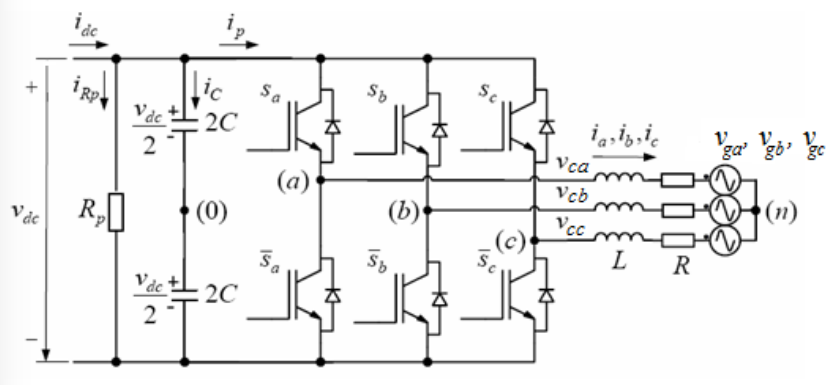
\includegraphics[width=.8\linewidth]{Images/FullConvFig.png}
    \caption{Three-phase inverter connected to the grid}
    \label{ModelFig}
  \end{figure}

  \begin{figure}[H]
    \centering
    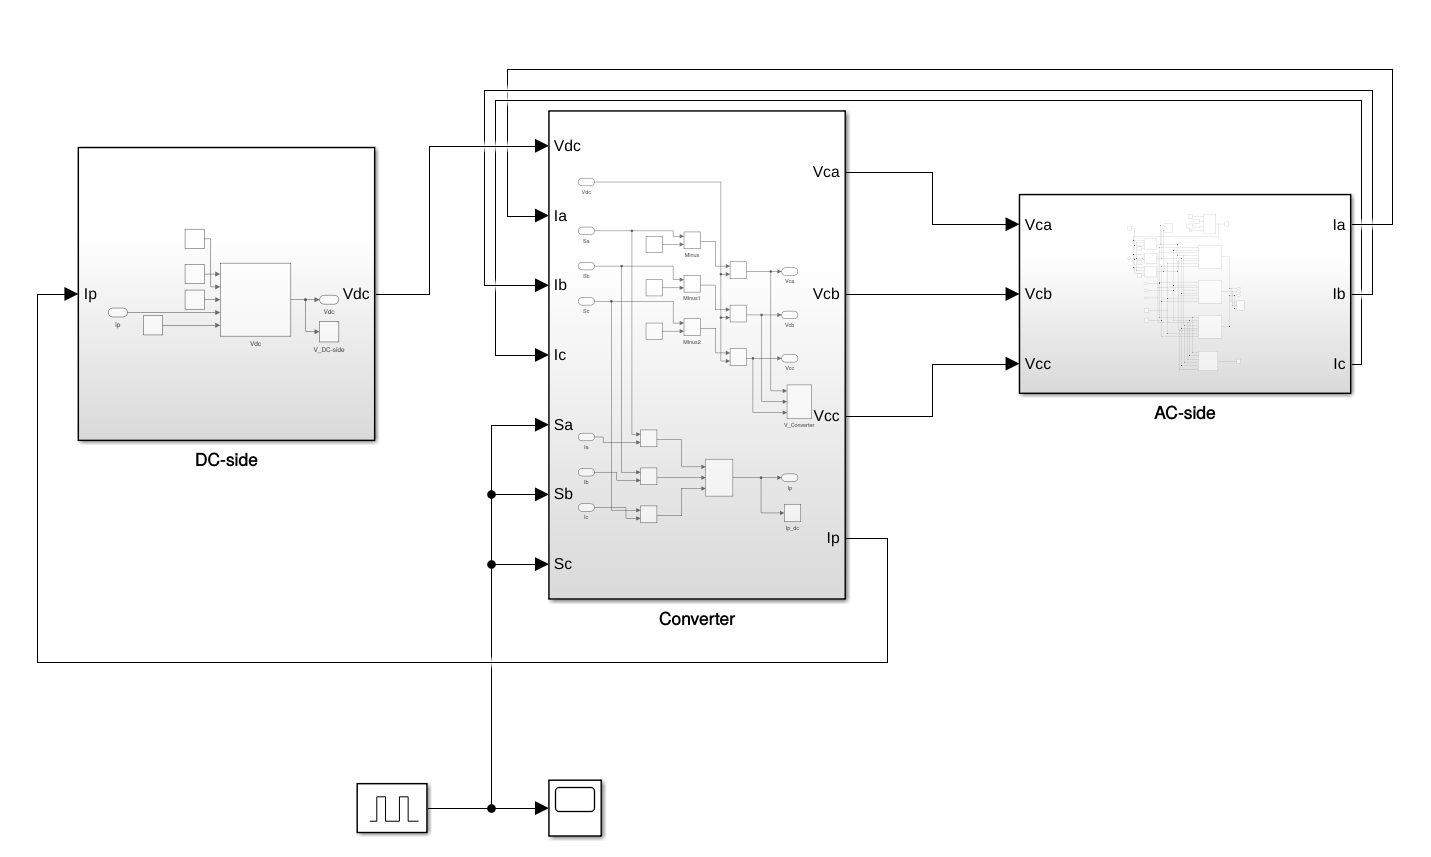
\includegraphics[width=.8\linewidth]{Images/S1Model.png}
    \caption{Final model after the first lab session}
    \label{S1Model}
  \end{figure}

\chapter{Modelling the AC side}

  The AC-side consists of a RL filter connected to an AC grid of 400V RMS 50Hz. The grid model includes a mechanism to drop the voltage for a certain amount of time in order to simulate a fault on the grid, the simulated fault is a three-phase fault with a 50\% depth during 5.5 cycles (or 110ms).\\

  The RL filter is used to filter out high frequencies generated by the power converter switching.\\

  \begin{figure}[H]
    \centering
    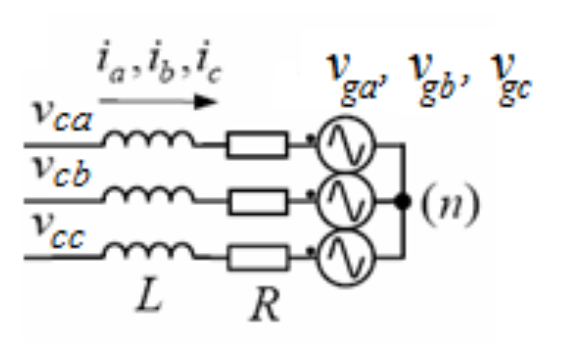
\includegraphics[width=.35\linewidth]{Images/AC-side_fig.png}
    \caption{AC-side of a three-phase inverter (RL filter + grid)}
    \label{AC-side_fig}
  \end{figure}

  \begin{figure}[H]
    \centering
    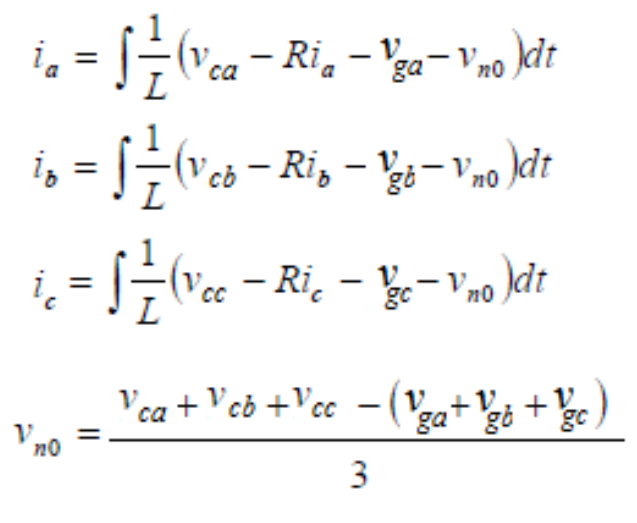
\includegraphics[width=.4\linewidth]{Images/AC-side_eq.png}
    \caption{Mathematical model for the AC-side}
    \label{AC-side_eq}
  \end{figure}

  \begin{figure}[H]
    \centering
    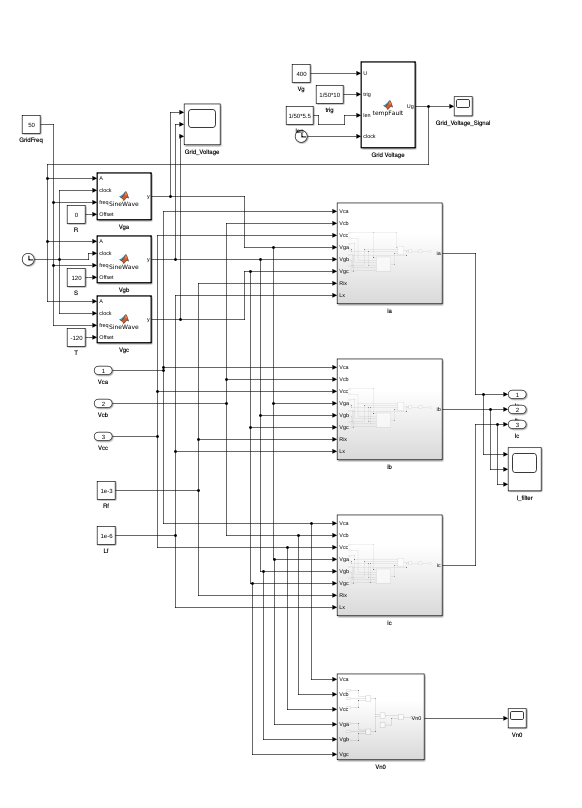
\includegraphics[width=.6\linewidth]{Images/AC-side_Simulink.png}
    \caption{Mathematical model for the AC-side translated into Simulink}
    \label{AC-side_Simulink}
  \end{figure}

  \begin{figure}[H]
      \centering
      \subfloat[Grid voltage simulated fault]{{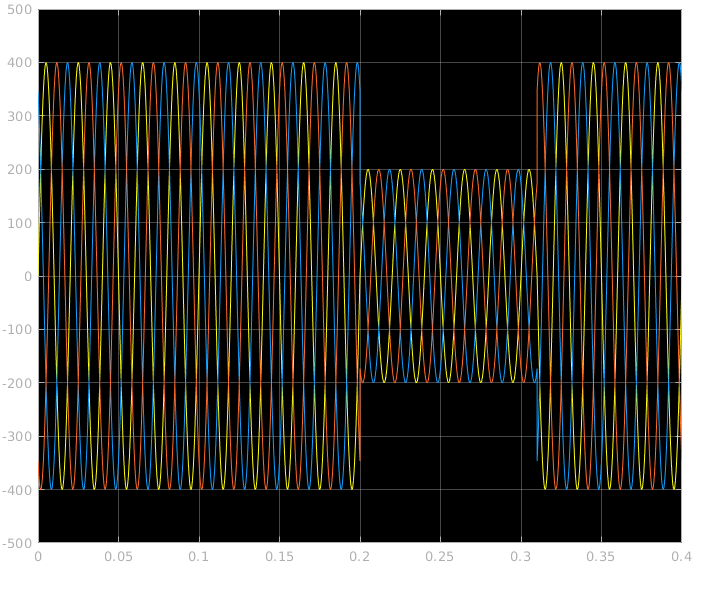
\includegraphics[width=.45\linewidth]{Images/Grid3Phase.png} }}%
      \qquad
      \subfloat[Voltage command signal drop]{{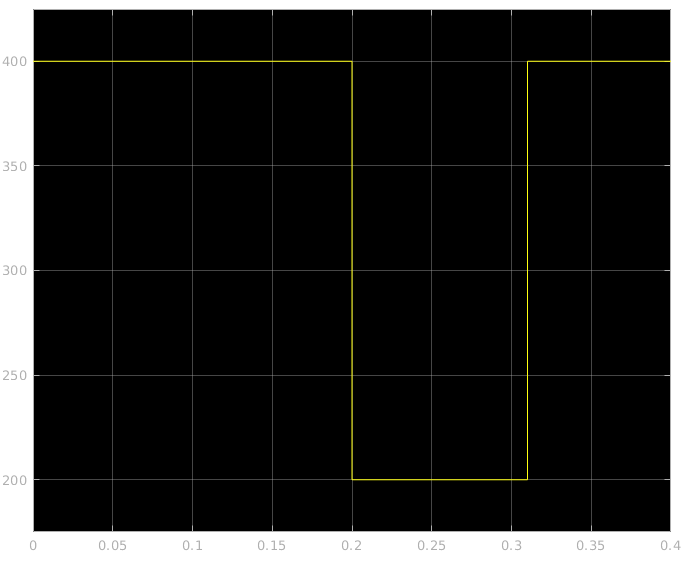
\includegraphics[width=.45\linewidth]{Images/GridV.png} }}%
      \caption{Three-phase grid fault}%
      \label{fig:example}%
  \end{figure}

\chapter{Modelling the DC side}

  The DC link of the power converter has also been modeled using a DC source in paralel with a resistor and a capacitor.\\

  \begin{figure}[H]
    \centering
    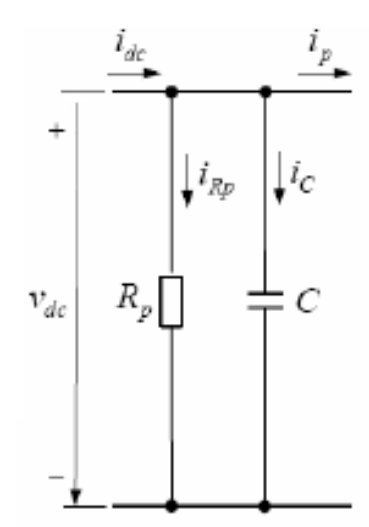
\includegraphics[width=.35\linewidth]{Images/DC-side_fig.png}
    \caption{DC-link of a three-phase inverter}
    \label{DC-side_fig}
  \end{figure}

  \begin{figure}[H]
    \centering
    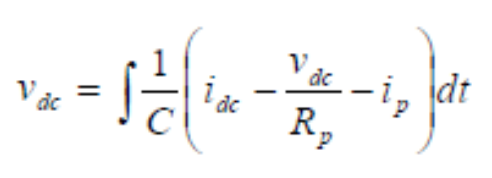
\includegraphics[width=.4\linewidth]{Images/DC-side_eq.png}
    \caption{Mathematical model for the DC-side}
    \label{DC-side_eq}
  \end{figure}

  \begin{figure}[H]
    \centering
    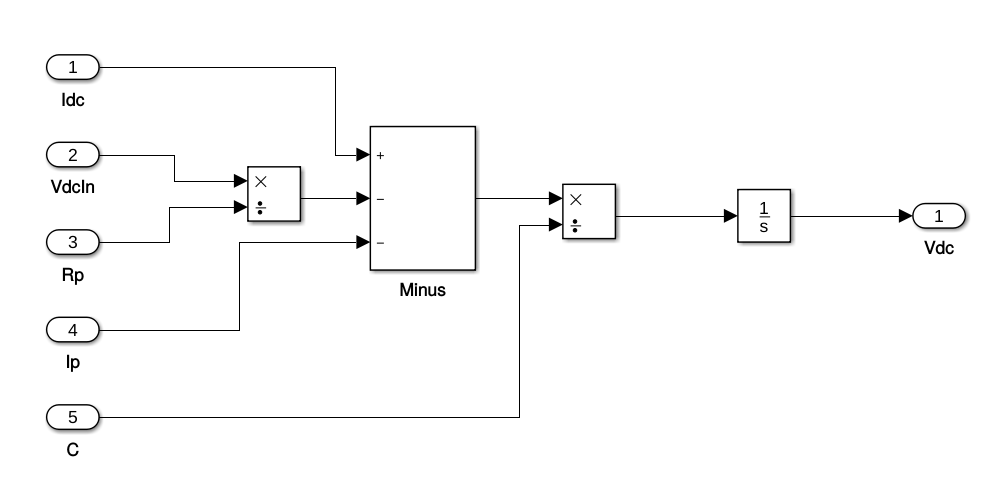
\includegraphics[width=.9\linewidth]{Images/DC_model.png}
    \caption{Mathematical model for the DC-side translated into Simulink}
    \label{DC-side_Simulink}
  \end{figure}


\chapter{Modelling the converter}

  Finally, the power converter has also been modeled, but control will be implemented on the next session.

  \begin{figure}[H]
    \centering
    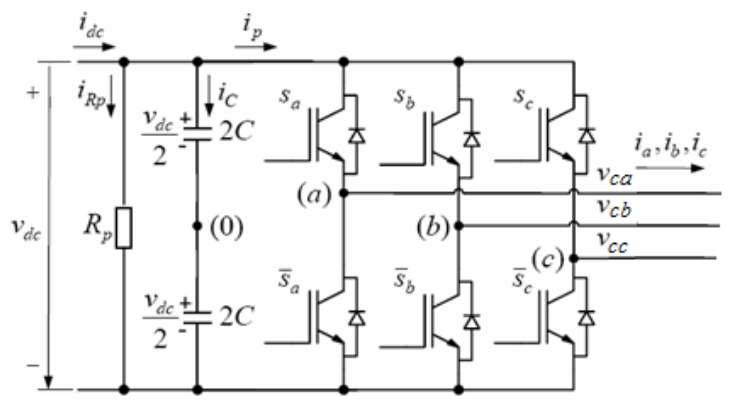
\includegraphics[width=.55\linewidth]{Images/Converter_fig.png}
    \caption{Three-phase inverter with IGBTs and diodes in anti-parallel}
    \label{Converter_fig}
  \end{figure}

  \begin{figure}[H]
    \centering
    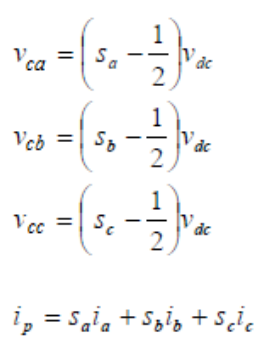
\includegraphics[width=.3\linewidth]{Images/Converter_eq.png}
    \caption{Mathematical model for converter}
    \label{Converter_eq}
  \end{figure}

  \begin{figure}[H]
    \centering
    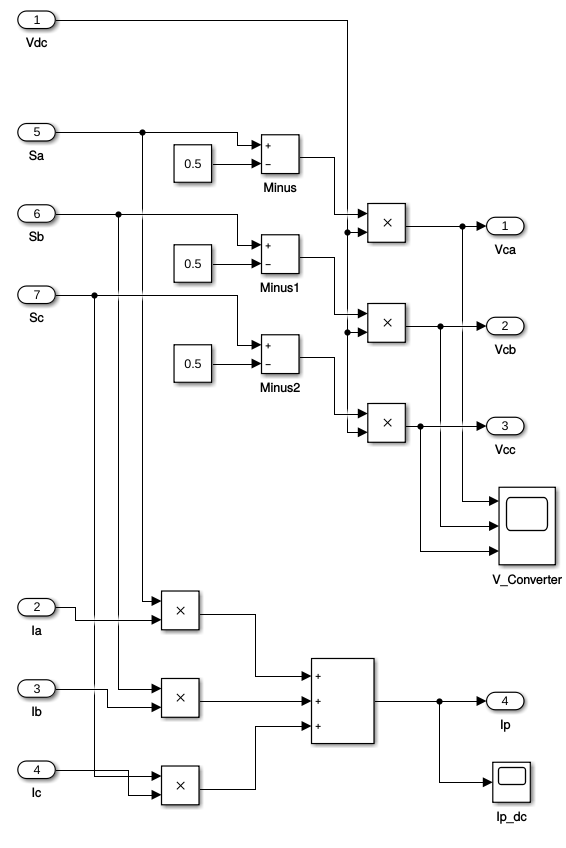
\includegraphics[width=.6\linewidth]{Images/ConverterSimulink.png}
    \caption{Mathematical model for the converter translated into Simulink}
    \label{Converter_Simulink}
  \end{figure}
